\chapter{Training e Testing del BDT}

\section{I Dati inziali}

I dati utilizzati per l'analisi svolta sono relativi a collisioni di due fasci di protoni incidenti al Cern. I dati, racccolti nel 2017 da ALICE, sono caratterizzati da un valore di $\sqrt{s} = 5 \ TeV$ \footnote{s è il quadrato della massa invariante della collisione, definita come $s = E^2 - \bar p ^2$} e sono relativi a 985 milioni di collisioni.
\\Da questi dati si vogliono selezionare solo le $D^{*+}$, che sono state ricostruite dal decadimento $D^{*+} \rightarrow D^0 + \pi^+ $ di cui si è parlato nel \ref{mesoneD}. Per fare ciò, ai dati utilizzati sono già state applicate delle pre-selezioni estremamente morbide che permettono di preservare praticamente tutto il segnale e di fare una prima scrematura dei dati grezzi.
A questo punto tutta l'analisi che segue è stata svolta considerando i dati suddivisi in vari intervalli. La suddivisione è basata sul valore del $p_T$, che è il valore del momento trasverso, ovvero il momento nella direzione perpendicolare a quella dei fasci di particelle incidenti. Gli intervalli di $p_T$ inizialmente considerati sono: [1,2], [2,3], [3,4], [4,5], [5,6], [6,8], [8,12], [12,16], [16,24] misurati in GeV/c. 
\\Per poter visualizzare i dati si possono considerare gli istogrammi della massa della $D^{*+}$, nel nostro caso si è scelto di utilizzare gli istogrammi della differenza in massa tra la $D^{*+}$ e la $D^0$ prodotta nel decadimento. Questa differenza in massa non è altro che la massa del $\pi^+$ relativo al primo decadimento, anche detto soft pi, che è il pione con momento più basso (rispetto al $\pi^+$ prodotto nel decadimento della $D^0$) ed è misurata in $Gev/c^2$. %Come mai usiamo gli istogrammi della differenza in massa e non direttamente quelli della massa della Dstar??
Di seguito si riportano gli istogrammi relativi ad alcuni intervalli di $p_T$, quelli relativi ai restanti intervalli di $p_T$ si trovano in appendice. 

    \begin{figure}[htbp]
        \centering
        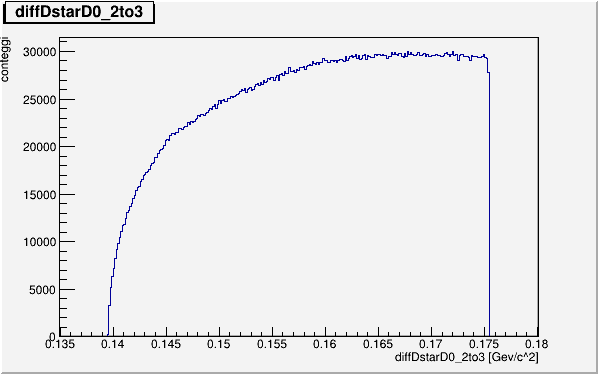
\includegraphics[width=0.7\linewidth]{training&testing/diffDstarD0_2to3.png}
        \caption{Distribuzione dei dati in funzione della differenza di massa tra la $D^*+$ e la $D^0$ per l'intervallo di $p_T$ [2,3]}
        \label{fig:grafmassDstar1}
    \end{figure}
    
Come si può vedere dal grafico \ref{fig:grafmassDstar1} non si evidenzia nessun picco evidente, cosa che ci si aspetta nel caso di una risonanza come la $D^{*+}$.\footnote{Una risonanza è una particella che ha un tempo di vita così corto da non essere direttamente osservabile e la cui esistenza si evidenzia considerando i prodotti del suo decadimento. In questo caso c'è un aumento della probabilità di trovare i prodotti del decadimento della risonanza in corrispondenza del valore della massa invariante della risonanza stessa} Questo accade perchè il numero di $D^{*+}$ prodotte è troppo piccolo rispetto al fondo di altre particelle e pertanto il picco della $D^{*+}$ non è riconoscibile rispetto al background.

    \begin{figure}[htbp]
        \centering
        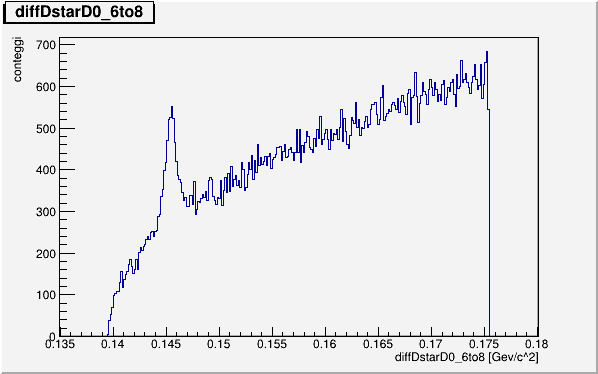
\includegraphics[width=0.7\linewidth]{training&testing/diffDstarD0_6to8.png}
        \caption{Distribuzione dei dati in funzione della differenza di massa tra la $D^*+$ e la $D^0$ per l'intervallo di $p_T$ [6,8]}
        \label{fig:grafmassDstar2}
    \end{figure}


Diversamente accade nel caso del grafico \ref{fig:grafmassDstar2} in cui si considera un intervallo di $p_T$ con valori del momento trasverso più alti. In questo caso il picco della $D^{*+}$ è già visibile e riconoscibile rispetto al fondo. 
Questa differenza tra le distribuzioni dei dati si riscontra per tutti gli intervalli di $p_T$ e tanto più è alto il $p_T$ tanto più è evidente il picco. Per ricostruire la $D^{*+}$ si considerano le combinazioni di tracce di due $\pi^+$ e un $K^-$ , ma a basso $p_T$ ci sono più combinazioni possibili mentre ad alto $p_T$ ce ne sono di meno. Pertanto per valori del momento trasverso più bassi le combinazioni errate, ovvero non relative alla $D^{*+}$ sono di più e quindi il fondo stesso è maggiore.

    \subsection{Le variabili di taglio}
    La selezione di tipo standard che viene svolta ad ALICE per il riconoscimento delle $D^{*+}$ è basata sulla scelta di alcune variabili di taglio e per ognuna di queste si sceglie un valore di \textit{taglio}. Le \textit{variabili di taglio} sono grandezze fisiche che descrivono il decadimento della $D^{*+}$ e che permettono di comprendere se le particelle considerate sono i prodotti di quel decadimento o meno. Il taglio, invece, è il valore scelto per discriminare tra segnale e fondo. 
    \\Anche per utilizzare il metodo del BDT sono state scelte alcune variabili di taglio, da cui, poi, l'algoritmo del BDT ha ricavato un'unica variabile finale: il textit{classifier output}. Solo per quest'ultima variabile è stato scelto un valore di taglio in base a cui selezionare le candidate $D^{*+}$. 
    Le variabili di taglio che possono essere considerate sono le seguenti:
        \begin{itemize}
            \item \textbf{massa$\bm{D^{*+}}$} è la massa della $D^{*+}$
            \item \textbf{massa$\bm{D^0}$} è la massa della $D^0$
            \item \textbf{diff$\bm{D^{*+}D^0}$} è la differenza tra la massa della  $D^{*+}$ e della $D^0$
            \item \textbf{$\bm{p_TD^{*+}}$} è il momento trasverso della $D^{*+}$
            \item \textbf{$\bm{{p_T\pi^+}_{soft}}$} è il momento trasverso del $\pi^+$ soft
            \item \textbf{$\bm{p_T\pi^+}$} è il momento trasverso del $\pi^+$ soft 
            \item \textbf{$\bm{p_TK^-}$} è il momento trasverso del $K^-$
            \item \textbf{$\bm{\eta}$} è l'angolo tra la direzione dei fasci di protoni incidenti e la direzione in cui è prodotta la $D^*+$ %Controllare se è giusto!!!
            \item \textbf{dist$\bm{K^-}$} è la distanza tra la traiettoria del Kaone $K^-$ e il vertice primario (PV) % \footnote{Il vertice primario è il punto in cui decade la $D^*+$}
            \item \textbf{dist$\bm{\pi^+}$} è la distanza tra la traiettoria del $\pi^+$ (prodotto dal decadimento della $D^0$) e il PV
            \item \textbf{distdist} è il prodotto dist$\pi^+$ per dist$K^-$
            \item \textbf{DCA} ovvero Distance of Closest Approach, è la distanza minima tra le traiettore del $K^-$ e del $\pi^+$, in teoria questa distanza dovrebbe essere nulla, in quanto le due traiettorie si dovrebbero incontrare nel vertice secondario (SV) %\footnote{Il vertice secondario è il punto in cui decade la $D^0$}.
            \item \textbf{cos$\bm{\theta_P}$} è il coseno dell'angolo di pointing. Quest'ultimo è l'angolo tra la retta congiungente il PV e il SV e la direzione del $p_T$ della $D^{*+}$.
             \item \textbf{cos$\bm{\theta_{P_{XY}}}$} è la proiezione del cos$\theta_P$ sul piano perpendicolare alla direzione dei fasci di protoni
            \item \textbf{cos$\bm{\theta^*}$} 
            \item \textbf{cos$\bm{\bar \theta^*}$}
            \item $\bm{\theta}$ 
            \item $\bm{L_{DECAD}}$ è la distanza di volo (ovvero la lunghezza di decadimento) della $D^0$ normalizzata per il suo errore 
             \item $\bm{L_{{DECAD}_{XY}}}$ è la proiezione della $\bm{L_{DECAD}}$ sul piano perpendicolare alla direzione dei fasci di protoni
        \end{itemize}{}
       
        
   Queste sono le variabili di taglio scelte inizialmente per il training del BDT. Dalle \textit{simulazioni Monte Carlo} si può vedere che queste variabili hanno una distribuzione diversa nel caso si consideri il segnale o il fondo. Proprio in base a queste differenze l'algoritmo utilizzato per questa analisi costruisce il BDT fornendo, alla fine del training, il classifier output. Si riportano di seguito i grafici delle distribuzioni di alcune di queste variabili per i dati (ottenuti da ALICE), per la simulazione del segnale e per la simulazione del fondo (ottenuti da simulatore MonteCarlo).
   
    \begin{figure}[htbp] %inserire grafici cca 4 variabili di taglio
        \centering
        \includegraphics[width=0.7\linewidth]{training&testing/variabilitaglio.png}
        \caption{}
        \label{fig:variabilitaglio}
    \end{figure}
   
   
    Durante la fase iniziale, si è provato il training del BDT utilizzando diversi set di variabili di taglio. In particolare si è considerata la correlazione tra le variabili, che può peggiorare i risultati degli algoritmi di analisi multivariata. Si è quindi scelto di non considerare le variabili fortemente correlate tra loro, dato che, nel caso in analisi, eliminare queste variabili non va a diminuire l'efficienza dell'algoritmo di training. 
    \\
    
    \begin{minipage}{.5\textwidth}%{0.5 cm} 
        \begin{flushleft} \large
        \flushleft
        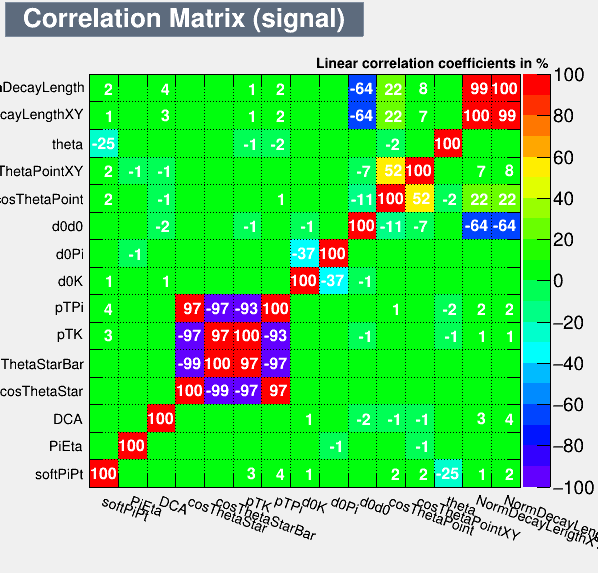
\includegraphics[width=7.5cm]{training&testing/CorrelationMatrixSin.png}
        \captionof{figure}{Griglia che mostra la correlazione lineare in percentuale tra le variabili di taglio considerate inizialmente per il training del segnale (da simulazione Monte Carlo)}
        \label{fig:correlazInizialeS}
        \end{flushleft}
        \end{minipage}
    ~
    \begin{minipage}{0.5\textwidth}
        \begin{flushright} 
        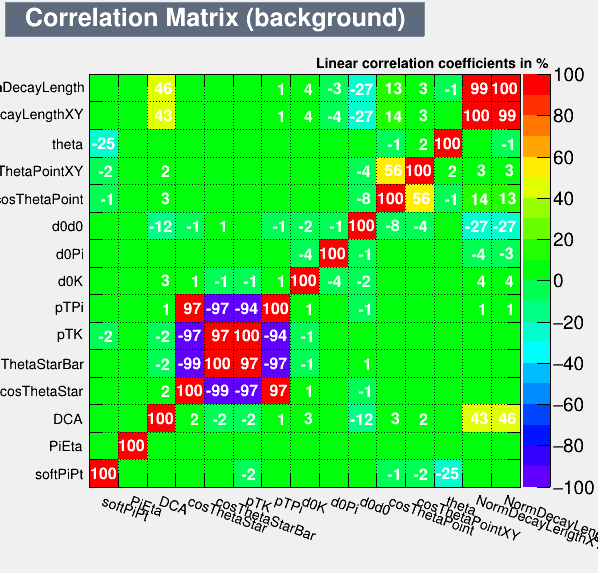
\includegraphics[width=7.5cm]{training&testing/CorrelationMatrixBin.png}
        \captionof{figure}{Griglia che mostra la correlazione lineare in percentuale tra le variabili di taglio considerate inizialmente per il training del fondo (da simulazione Monte Carlo)}
        \label{fig:correlazInizialeB}
        \end{flushright}
    \end{minipage}\\[0.5cm]
    
 %   \begin{figure}[htbp] %grafico correlazione lineare tutte variabili
 %       \centering
 %       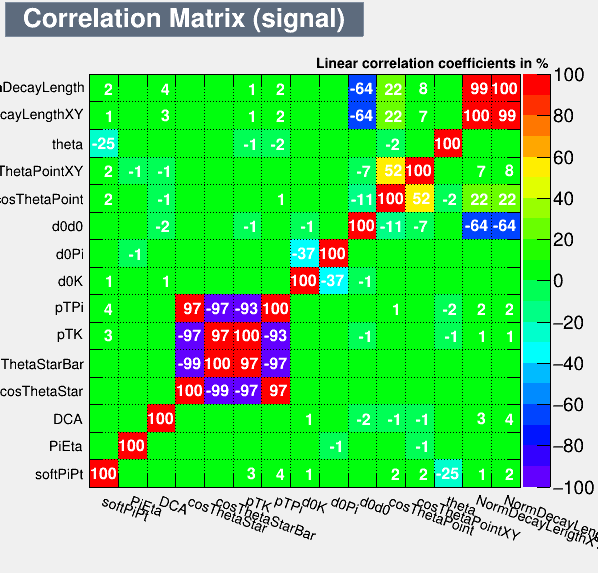
\includegraphics[width=0.7\linewidth]{training&testing/CorrelationMatrixSin.png}
%        \caption{Griglia che mostra la correlazione lineare in percentuale tra le variabili di taglio considerate inizialmente per il training per il segnale (da simulazione Monte Carlo)}
%        \label{fig:correlazInizialeS}
%    \end{figure}
    
    
%     \begin{figure}[htbp] %grafico correlazione lineare tutte variabili
%        \centering
%        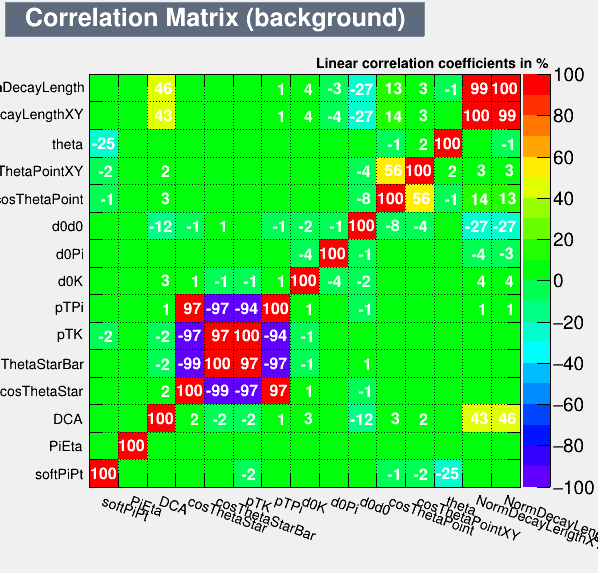
\includegraphics[width=0.7\linewidth]{training&testing/CorrelationMatrixBin.png}
%        \caption{Griglia che mostra la correlazione lineare in percentuale tra le variabili di taglio considerate inizialmente per il training per il fondo (da simulazione Monte Carlo)}
%        \label{fig:correlazInizialeB}
%    \end{figure}
    
    
    Inoltre si è deciso di aggiungere anche la \textit{Particle Identification} (PID), che ha permesso di ottenere risultati migliori nella fase di analisi dei dati di ALICE. La PID sfrutta i dati relativi alla perdita di energia delle particelle all'interno del rivelatore: $\frac{dE}{dx}$. Conoscendo la carica della particella e le caratteristiche del materiale di cui è composto il rivelatore, si può utilizzare la \textit{Bethe-Bloch}. Confrontando i dati della perdita di energia con la Bethe-Bloch si può ricavare la massa della particella e quindi identificare la particella stessa. In pratica le limitazioni dovute alle fluttuazioni statistiche e alla precisione dei rivelatori non permettono un'identificazione certa ma di tipo statistico. 
    \\Allo stesso modo è stato utilizzato anche il \textit{Time Of Flight} (TOF), ovvero la misura del tempo impiegato dalla particella a percorrere una determinata lunghezza nel rivelatore. Conoscendo la lunghezza considerata e il momento della particella si può ricavare la massa della particella stessa. Anche in questo caso le stesse limitazioni della PID impediscono un'identificazione diretta e certa della particella. 
    
    \begin{figure}[htbp]
        \centering
        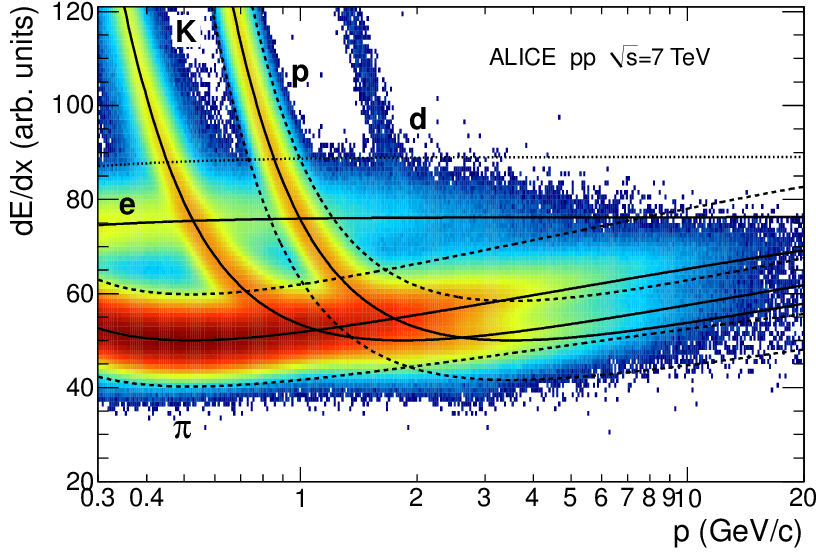
\includegraphics[width=0.6\linewidth]{training&testing/Specific-energy-loss-in-the-TPC.png}
        \caption{ Perdita di energia specifica nella TPC (\ref{TPC}) in funzione del momento, sono riportati anche gli andamenti della Bethe-Bloch per vari tipi di particelle.}
        \label{fig:BBnellaTPC}
    \end{figure}
    
    Come si vede dalla figura \ref{fig:BBnellaTPC}, i dati non possono sempre essere ricondotti univocamente all'andamento di una singola particella. Nell'analisi relativa a questa tesi si è considerata la differenza tra la $\frac{dE}{dx}\mid_m$ misurata dalla TPC e la $\frac{dE}{dx}\mid_{th}$ calcolata con la Bethe-Bloch, il tutto rinormalizzato per la risoluzione della TPC. 
    \\Allo stesso modo è stata utilizzata anche la differenza tra il $TOF\mid_{m}$ misurato con il rivelatore TOF e il $TOF\mid_{th}$ calcolato terociamente, tutto rinormalizzato per la risoluzione del rivelatore TOF.
    
    Le variabili di taglio aggiunte sono:
    \begin{itemize}
        \item $\bm{TPC_{PID,\pi^+}}$: $(\frac{dE}{dx}\mid_{m, \pi} \ - \ \frac{dE}{dx}\mid_{th, \pi} ) / \sigma_{TPC} \ $ per il $\pi^+$ prodotto dal decadimento della $D^0$ %nSigmaTPCpi
        \item $\bm{TPC_{PID,K^-}}$ :  $(\frac{dE}{dx}\mid_{m,K} \ - \ \frac{dE}{dx}\mid_{th,K} ) / \sigma_{TPC} \ $ per il $K^-$ prodotto dal decadimento della $D^0$ %nSigmaTPCK
        \item $\bm{TOF_{PID,\pi^+}}$ : $ (TOF\mid_{m,\pi} \ - \ TOF\mid_{th,\pi}) / \sigma_{TOF} \ $ per il $\pi^+$ prodotto dal decadimento della $D^0$ %nSigmaTOFpi
        \item $\bm{TOF_{PID,K^-}}$ : $ (TOF\mid_{m,K} \ - \ TOF\mid_{th,K}) / \sigma_{TOF} \ $ per il $K^-$ prodotto dal decadimento della $D^0$ %nSigmaTOFK
    \end{itemize}{}
    
    La correlazione tra le variabili di taglio scelte per l'analisi dei dati finale di ALICE è minima per tutte le variabili, ad eccezione delle variabili $L_{{DECAD}_{XY}}$ , distdist, e DCA, come si vede dalle figure \ref{fig:correlazFinaleS} e \ref{fig:correlazFinaleB}
    \\
   
      \begin{minipage}{.5\textwidth}%{0.5 cm} 
        \begin{flushleft} \large
        \flushleft
        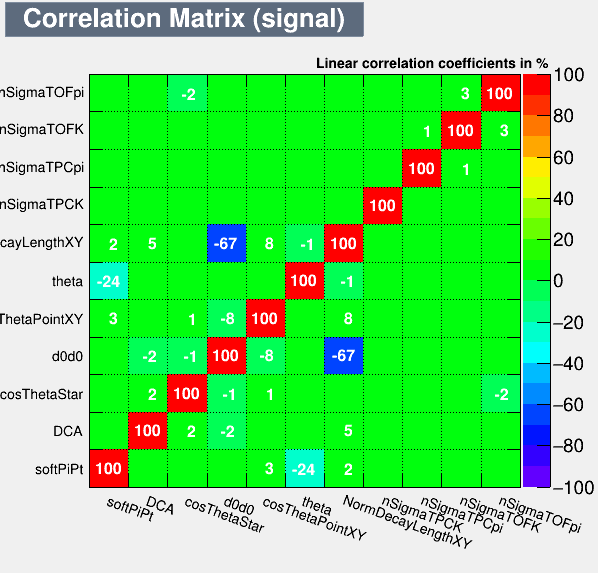
\includegraphics[width=7.5cm]{training&testing/CorrelationMatrixS.png}
        \captionof{figure}{Correlazione lineare in percentuale tra le variabili di taglio considerate per il training finale del segnale (da simulazione Monte Carlo)}
        \label{fig:correlazFinaleS}
        \end{flushleft}
        \end{minipage}
    ~
    \begin{minipage}{0.5\textwidth}
        \begin{flushright} \large
        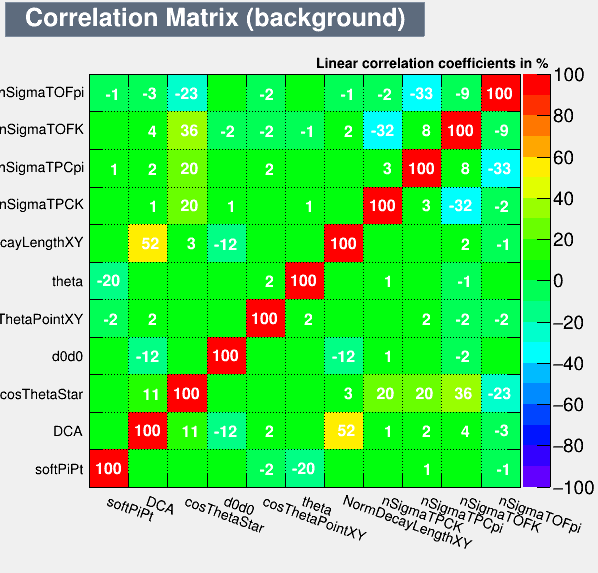
\includegraphics[width=7.5cm]{training&testing/CorrelationMatrixB.png}
        \captionof{figure}{Correlazione lineare in percentuale tra le variabili di taglio considerate per il training finale del fondo (da simulazione Monte Carlo)}
        \label{fig:correlazFinaleB}
        \end{flushright}
    \end{minipage} \\[1.cm]
    
%        \begin{figure}[htbp] %grafico correlazione lineare variabili finali
%        \centering
%        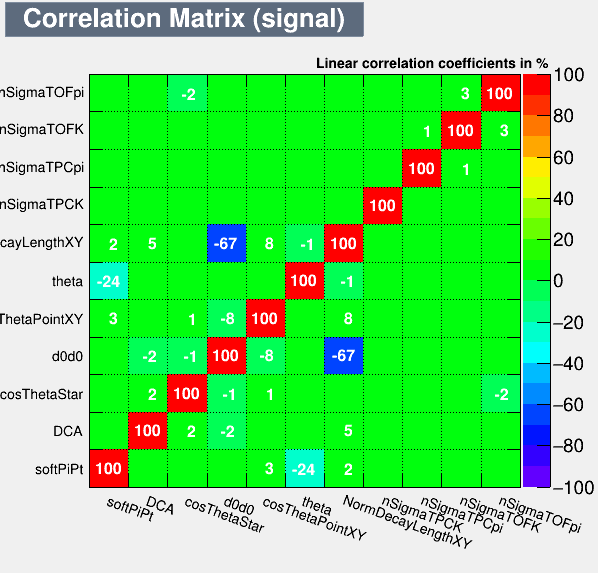
\includegraphics[width=0.7\linewidth]{training&testing/CorrelationMatrixS.png}
%        \caption{Correlazione lineare in percentuale tra le variabili di taglio considerate per il training finale del segnale (da simulazione Monte Carlo)}
%        \label{fig:correlazFinaleS}
%    \end{figure}
    
%    \begin{figure}[htbp] %grafico correlazione lineare variabili finali
%        \centering
%        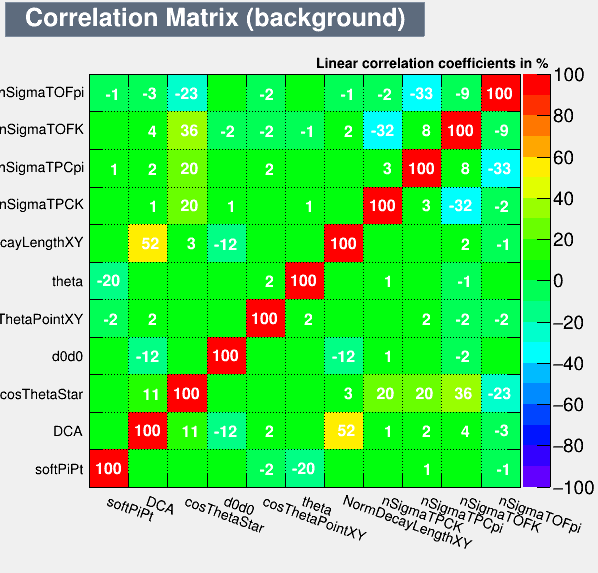
\includegraphics[width=0.7\linewidth]{training&testing/CorrelationMatrixB.png}
%        \caption{Correlazione lineare in percentuale tra le variabili di taglio considerate per il training finale del fondo (da simulazione Monte Carlo)}
%        \label{fig:correlazFinaleB}
%    \end{figure} 
    
    
  
  
\section{Training}

\subsection{Scelta dei dati per il training}
Come si è detto in precedenza per il training del BDT si sono utilizzati dati provenienti da \textit{simulazioni Monte Carlo}. Queste permettono, infatti, di simulare la collisione di fasci di protoni e quindi le particelle che vengono create. I dati forniti dal Monte Carlo, però, non sono del tutto aderenti alla realtà fisica prodotta nell'esperimento di LHC, specialmente se si considera il fondo. 
\\ Inizialmente si sono utilizzati i dati delle simulazioni Monte Carlo ma per cercare di descrivere meglio il fondo si è deciso di considerare per la parte del \textit{segnale} i dati provenienti da simulazione Monte Carlo, mentre per il \textit{fondo} i dati dell'esperimento ALICE. È quindi necessario riuscire a selezionare dagli istogrammi dei dati di ALICE in funzione della diff${D^{*+}D^0}$ ( come il grafico \ref{fig:grafmassDstar1}) solamente il fondo senza prendere anche parte del segnale. Per fare questo si è scelto un valore minimo della variabile diff${D^{*+}D^0}$ e si sono presi solo i dati a destra di tale valore. Per scegliere il valore minimo si sono utilizzati sia il valore della massa del $\pi^+$ (che è la differenza tra la massa della $D^{*+}$ e della $D^0$), sia gli istogrammi dei dati di ALICE per alti intervalli di $p_T$ in cui il picco è più facilmente distinguibile (\ref{fig:grafmassDstar1}), sia i primi risultati ottenuti dall'analisi che era stata già terminata utilizzando solo simulazioni Monte Carlo per il training e in cui era in parte distinguibile il picco del segnale anche per $p_T$ più bassi. Il valore scelto come limite inferiore è di $147.8 \ MeV/c^2$, che evidentemente più alto della massa del $\pi^+$ $139.5 \ MeV/c^2$.
\\A questo punto non ci sono più dati per il training che descrivono il fondo a sinistra del picco, infatti in questo intervallo della diff${D^{*+}D^0}$ non è possibile individuare i dati di ALICE corrispondenti solo al fondo e non al segnale come fatto prima. L'analisi dei dati di ALICE  ottenuta in questo modo, non distingueva bene il segnale dal fondo nella parte sinistra del picco, evidenziando la difficoltà dell'algoritmo nel selezionare le $D^{*+}$ in assenza di dati per il training in quel particolare intervallo. 
\\Per risolvere questo problema si è deciso di utilizzare i dati della simulazione Monte Carlo per il fondo a sinistra del picco del segnale. I dati del fondo della simulzione Monte Carlo, pur non descrivendo al meglio i dati reali di ALICE, hanno fornito comunque una base per il training del BDT nella parte a sinistra del picco del segnale ed hanno permesso di ottenere risultati migliori nel riconoscimento delle $D^{*+}$. 
\\In figura \ref{fig:dati_training} è riportato il grafico dei dati utilizzati per il training per l'intervallo di $p_T$ [3-4]. Si vede in blu il segnale generato con simulazione Monte Carlo, in rosso il fondo a sinistra generato con simulazione Monte Carlo e in verde il fondo a destra preso dai dati di ALICE. Come si nota in \ref{fig:dati_training} i dati del fondo a destra non ci sono per valori alti della diff${D^{*+}D^0}$, questo semplicemente perchè l'analisi per distinguere segnale da fondo è rivelante solo nell'intorno del piccodi segnale, mentre dove mancano i dati per il training siamo già sicuri sia solo fondo. 


    \begin{figure}[htbp] 
        \centering
        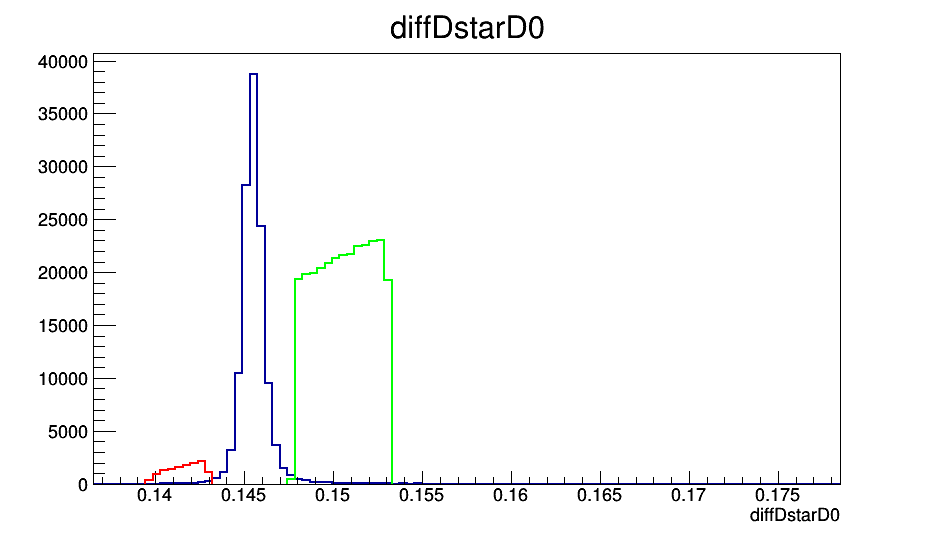
\includegraphics[width=0.9\linewidth]{training&testing/diffDstarD0_training_3_4_ok.png}
        \caption{Dati utilizzati per il training per l'intervallo di $p_T$ [3-4]: in blu il segnale, in rosso il fondo a sinistra ed in verde il fondo a destra }
        \label{fig:dati_training}
    \end{figure}
    
    
    

\subsection{Scelta dei Parametri del BDT}
L'algoritmo del BDT ha al suo interno alcuni parametri che possono essere variati e che possono cambiare le performance dell'algoritmo nel risolvere il problema. Per l'analisi svolta in questa tesi sono stati considerati nello specifico solo due parametri. Il primo è il \textit{numero di alberi} che compongono la "foresta" del BDT. Come spiegato nel paragrafo \ref{BDT}  il training viene fatto su un grande numero di alberi il cui responso viene unito in un'unica variabile finale. Aumentando il numero di alberi l'efficienza dell'algoritmo migliora, finché non si raggiunge un plateau e i risultati dell'analisi non variano all'aumentare del numero di alberi. Dato che un maggiore numero di alberi della foresta significa maggiore tempo impiegato sia per il training che per l'analisi dei dati, si è cercato il numero minimo di alberi che restituisse i risultati migliori ottenibili.
\\Il numero standard di alberi della foresta è di 850, ma variando questo numero si è trovato che già per 300 alberi i risultati erano gli stessi. Pertanto nell'analisi finale, di cui si riporteranno i risultati nel capitolo seguente, l'algoritmo del BDT ha 300 alberi. 
\\Il secondo parametro considerato è la \textit{profondità massima} di ogni albero. Con profondità si intende il numero di livelli di un albero. Ad esempio, in figura \ref{fig:depthBDT} l'albero ha 3 livelli, perchè per arrivare dal nodo principale all'ultima foglia si incontrano 3 diverse diramazioni.
\\
    \begin{figure}[htbp] 
        \centering
        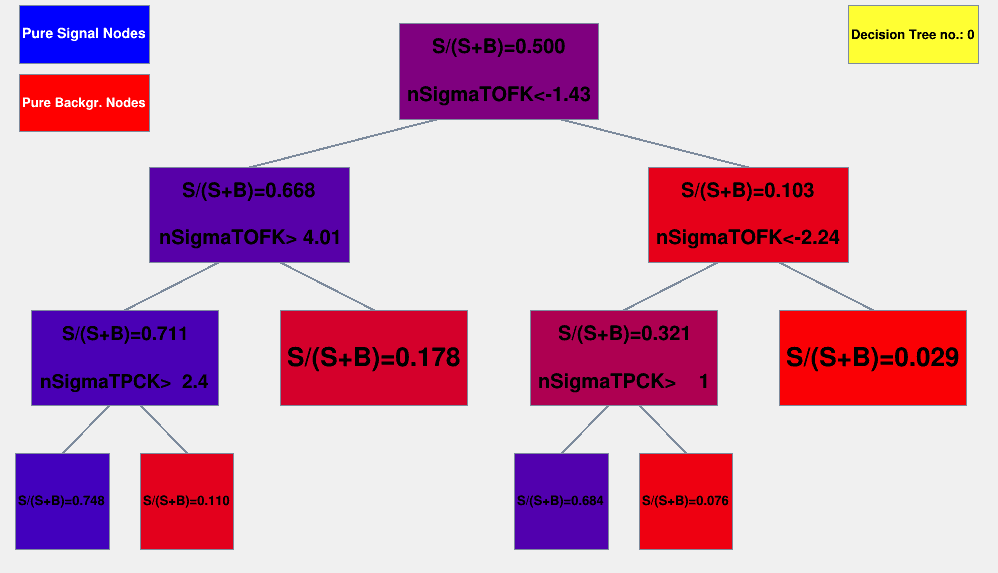
\includegraphics[width=0.7\linewidth]{training&testing/depthBDT.png}
        \caption{Schema di un albero del BDT con 3 livelli}
        \label{fig:depthBDT}
    \end{figure}
    
In questo caso si è visto che diminuendo la profondità massima a 2 livelli le performance dell'algoritmo peggiorano, mentre non c'è guadagno nell'aumentarla a 4. Dato che aumentando il numero massimo di livelli aumenta il tempo necessario per il training, l'analisi finale dei dati di ALICE è stata svolta con il parametro della profondità massima uguale a 3.

\subsection{I risultati del Training}

Alla fine del training della foresta di alberi,le caratteristiche di ogni albero, quindi i nodi di cui è composto, le variabili su cui si è discriminato, l'identificazione delle foglie come segnale o fondo, i pesi dei vari rami, vengono salvate in automatico. Questi valori vengono poi utilizzati per l'analisi dei dati di ALICE. 
\\Per valutare le performance dell'algoritmo del BDT utilizzato si possono considerare alcune grandezze, la prima è la \textit{ROC-Curve} (Receiving Operating Characteristics Curve) e in particolare l'area sottesa alla ROC-Curve. La ROC-Curve è il grafico della background rejection in funzione della signal efficiency. Dove la background rejection è 1 - background efficiency, la background efficiency è il numero di eventi del fondo selezionati come fondo e la signal efficiency è il numero di eventi segnale selezionati come segnale.
Un algoritmo è tanto più efficiente quanto più è alto il valore dell'area della Roc-Curve. %, il cui  limite teorico è fissato dal Likelihood Ratio.
Riportiamo in figura \ref{fig:RocCurve} il grafico della ROC-Curve relativa al training del bin di $p_T$ [3-4] con 300 alberi con profondità massima 3. In questo caso l'area sottesa alla curva è ROC-integral = 0.945 . 
    \begin{figure}[htbp] 
        \centering
        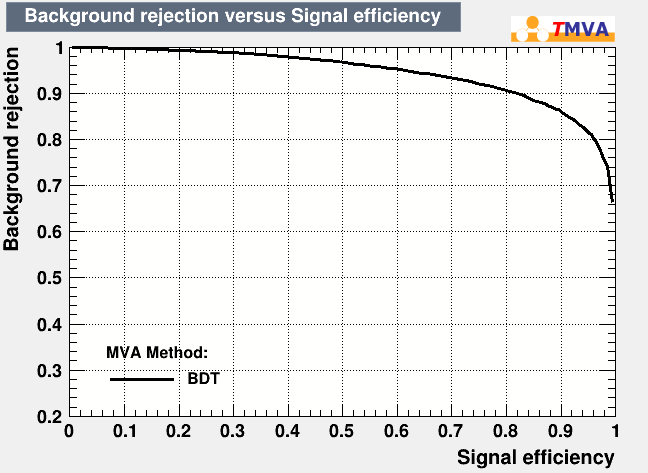
\includegraphics[width=0.7\linewidth]{training&testing/RocCurve.png}
        \caption{Grafico della ROC-Curve relativa al training del BDT con 300 alberi e profondità massima 3}
        \label{fig:RocCurve}
    \end{figure}
    
Un'altra grandezza da considerare è la distribuzione dei dati in funzione del classifier output (di cui si è parlato nel \ref{AnalisiMulti}), che in questo caso è chiamato \textit{BDTresponse}. Questo ci fornisce una prima indicazione di quanto sarà possibile separare il segnale dal fondo, infatti, laddove si sovrappongono non sarà possibile separare segnale e fondo quando si utilizzerà questo BDT sui dati di ALICE. Il grafico in figura \ref{fig:BDTresponse} mostra proprio la distribuzione dei dati del testing in funzione del BDTresponse. Si utilizzano i dati del testing (di cui si è parlato nel \ref{BDT}) per fare dei test sulle performance dell'algoritmo. 

    \begin{figure}[htbp] 
        \centering
        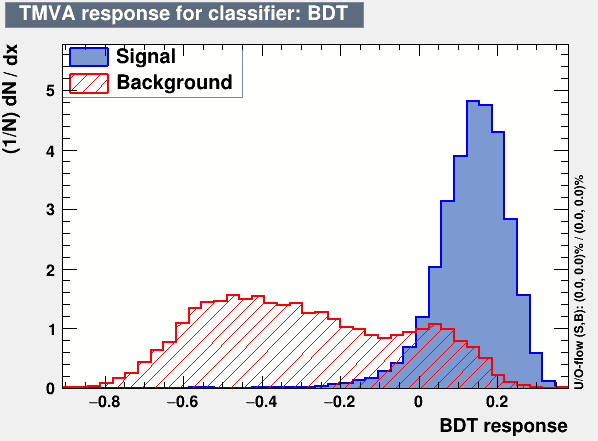
\includegraphics[width=0.7\linewidth]{training&testing/BDTresponsetest.png}
        \caption{Distribuzione dei dati del testing rispetto al BDTresponse del training con 300 alberi e profondità massima 3}
        \label{fig:BDTresponse}
    \end{figure}
    
Se confrontiamo la distribuzione dei dati in figura \ref{fig:BDTresponse} e quella rispetto alle variabili di taglio in figura \ref{fig:variabilitaglio}, si nota facilmente quanto la differenza tra la distribuzione del fondo e del segnale sia aumentata considerando il BDTresponse, piuttosto che le grandezze fisiche delle variabili di taglio. Questo è proprio il vantaggio offerto dall'analisi multivariata e nel caso specifico dall'algoritmo del BDT.
    
\\Infine è importante anche considerare l'\textit{efficienza del BDT}, che come detto in precedenza è il numero degli eventi segnale che sono stati classificati come segnale dall'algoritmo. Pertanto se l'efficienza è 1 tutti gli eventi segnale sono stati riconosciuti come tali, mentre se è 0 tutti gli eventi segnale sono stati classificati come fondo. Si deve notare, però, che anche nel caso in cui  l'efficienza sia 1 è possibile (anzi probabile) che alcuni eventi fondo siano stati classificati come segnale e perciò la selezione ha comunque dei problemi.
\\Per questo motivo si considerano anche altre grandezze quali l'efficienza del fondo e la significatività, quest'ultima è definita come 

    \begin{equation}
        s \ = \ \frac{eff_{segnale}}{\sqrt{eff_{segnale} + eff_{fondo}}}
    \end{equation}{}

Sia l'efficienza del segnale, che l'efficienza del fondo, che la significatività variano in base al valore del taglio applicato al valore del BDTresponse. Il taglio è il valore scelto come limite per dividere il segnale dal fondo, per esempio, considerando il grafico di figura \ref{fig:BDTresponse}, più il valore del taglio è alto più l'efficienza del segnale aumenta ma l'efficienza del fondo diminuisce. Si riporta in figura \ref{fig:effBDT} il grafico di queste grandezze al variare del valore del taglio per il training fatto con 300 alberi e profondità massima 3.
\\

    \begin{figure}[htbp] 
        \centering
        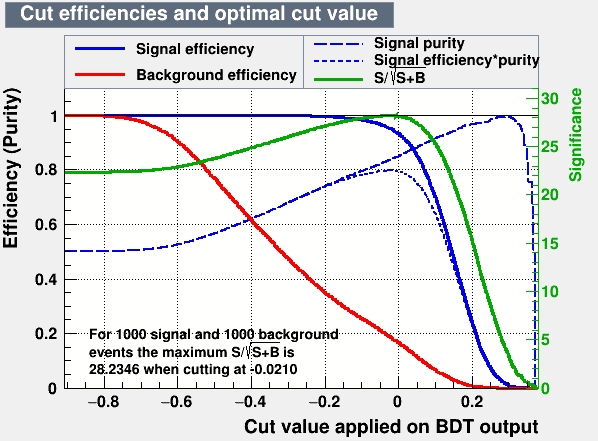
\includegraphics[width=0.7\linewidth]{training&testing/effBDT.png}
        \caption{Grafico dell'efficienza del segnale in blu, efficienza del fondo in rosso e significatività in verde, al variare del valore del taglio scelto per la BDTresponse. Gli andamenti sono relativi al training con 300 alberi e profondità massima 3}
        \label{fig:effBDT}
    \end{figure}
    
Attraverso le grandezze di cui si è appena parlato è quindi stato possibile fare delle verifiche sulle performance e sull'utilità dell'algoritmo del BDT per l'analisi dati che si vuole svolgere in questa tesi. In particolare si sono notati due problemi principali utilizzando il BDT. Da un lato per l'intervallo di $p_T$ [1,2], ovvero il più basso considerato in questa analisi, si sono subito riscontrati dei problemi.  In particolare il problema sta nel numero molto basso di eventi segnale nei dati della simulazione Monte Carlo. Ricordiamo, infatti, che a basso $p_T$ ci sono molti più eventi fondo rispetto al segnale, ma per il bin di $p_T$ che stiamo considerando gli eventi segnale appartenenti al dataset della simulazione usata per il training è molto basso, nel caso specifico si hanno appena $117$ eventi segnale (contro i circa $100000$ del fondo). 
\\A questo punto è fondamentale ricordare che i metodi di analisi basati sul Machine Learning funzionano bene quando si utilizzano grandi quantità di dati, infatti è proprio grazie ai numerosi esempi su cui viene fatto il training che l'algoritmo impara a riconoscere e selezionare le varie tipologie di dati. 
È quindi evidente il problema di utilizzare per il training solamente $90$ eventi per il segnale. In questo caso si è considerato circa l'$80\%$ dei 117 eventi totali per il training e il restante $20\%$ per il testing. Si riporta il grafico della distribuzione dei dati in funzione del BDTresponse. 

 \begin{figure}[htbp] 
        \centering
        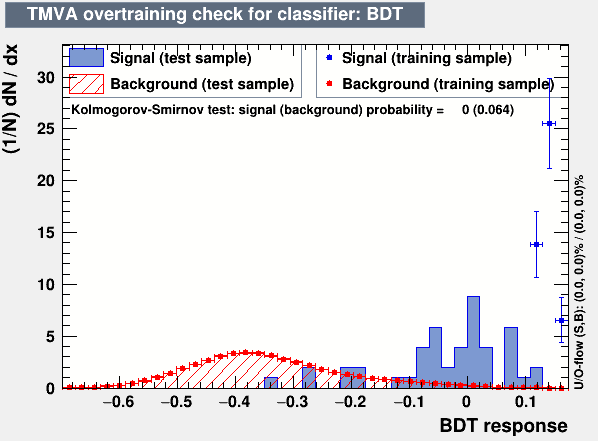
\includegraphics[width=0.7\linewidth]{training&testing/BDTresponse_0_1.png}
        \caption{Distribuzione dei dati di training e testing rispetto al BDTresponse del training con 300 alberi e profondità massima 3 per il bin di $p_T$ [0,1]. I rettangoli rappresentano i risultati del testing, i punti con i relativi errori i risultati del training.
        }
        \label{fig:BDTresponse_0_1}
    \end{figure}
    
Come si vede dal grafico \ref{fig:BDTresponse_0_1} la distribuzione dei dati del segnale del testing non è uniforme ed è molto sovrapposta a quella del fondo, questo rende difficile individuare un buon valore del taglio della BDTresponse e in generale poco efficace il metodo del BDT per la selezione delle $D^{*+}$. Inoltre si nota anche che le distribuzioni dei dati del training e del testing del segnale differiscono notevolmente fra loro. Come verrà spiegato più avanti nella sezione \ref{testing}, questo è un altro indice che il BDT non sta funzionando correttamente. Per questi motivi si è deciso di non continuare l'analisi per il bin di $p_T$ [0,1] ma solo per $p_T \ > 1 \  Gev/c$. 
\\Il secondo problema con l'utilizzo del BDT si è riscontrato per i bin di $p_T$ più alto, ovvero [12,16] e [16,24].  Il problema sta nel numero troppo basso di eventi, ovvero la statistica è troppo poca per permettere al BDT di funzionare correttamente, in questo caso specialmente per il fondo. Inoltre, si deve considerare che all'aumentare del $p_T$ il picco di segnale nella distribuzione dei dati di ALICE rispetto alla variabile $diffD^{*+}D^0$ diventa sempre più evidente e più facilmente individuabile anche con un'analisi che non utilizza metodi multivariati. Pertanto non è stata continuata l'analisi dati anche per valori di $p_T \ > \ 12 \ Gev/c$. 

%___________RIVEDERE ALTO PT________________________________-
%_________________________________________________
%___________________________________________________



\subsection{Scelta dei valori di taglio}

L'ultima operazione da compiere per concludere il training del BDT è quella di scegliere i valori di taglio della variabile BDTresponse, che permettono, poi, nella fase di analisi dei dati di ALICE di discriminare tra segnale e fondo. Per scegliere i valori di taglio si è fatto riferimento da una parte ai grafici delle efficienze e della significatività di cui si è parlato precedentemente, dall'altra si sono confrontati i risultati dell'analisi dei dati di ALICE (di cui si parla nel capitolo \ref{Analisi}) e come questi variano in base al taglio. 

Nell'utilizzare i grafici di efficienze e significatività per la scelta del valore di taglio è stato fondamentale aver considerato un rapporto segnale-fondo molto basso (10:1000), questo perchè nei dati di ALICE abbiamo che gli eventi segnale sono molti meno degli eventi fondo. In tal modo anche i risultati del training del BDT e le curve di efficienze e significatività sono più aderenti ai dati di ALICE.

    \begin{figure}[htbp] 
        \centering
        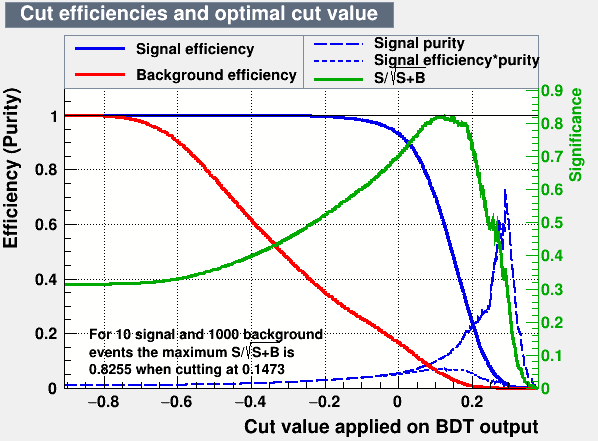
\includegraphics[width=0.7\linewidth]{training&testing/effBDT/effBDT_rapp_3_4.png}
        \caption{Grafico dell'efficienza del segnale in blu, efficienza del fondo in rosso e significatività in verde, al variare del valore del taglio scelto per la BDTresponse per il bin di $p_T$ [3,4]. Il rapporto tra segnale e fondo è di 10:1000 . Gli andamenti sono relativi al training con 300 alberi e profondità massima 3
        }
        \label{fig:effBDT_10_1000}
    \end{figure}
    
Una scelta per il valore di taglio inizialmente presa in considerazione è il punto di massimo della significatività. L'analisi dei dati di ALICE. però, è stata svolta anche per altri valori di taglio del BDTresponse è si è visto che abbassando di poco il valore di taglio la significatività dei dati di ALICE aumentava. In particolare si è scelto il punto in cui la curva dell'efficienza del segnale e quella della significatività si incontrano, cercando così di avere un buon compromesso tra la quantità di segnale selezionata e la significatività. Per i bin di $p_T$ più alti i grafici della significatività diventano sempre meno lineari. probabilmente a causa del diminuire della quantità di dati utilizzata per il training, pertanto in alcuni casi è stato scelto un valore di taglio più alto rispetto a quello del metodo precedentemente indicato. In appendice si riporatno i grafici di efficienze e significatività per tutti gli intervalli di $p_T$ considerati.
Nella prossima teabella si riportano i valori di taglio della BDTresponse per tutti gli intervalli di $p_T$ su cui è stata svolta l'analisi finale.

    \begin{table}[H]
		\centering
		\begin{tabular}{c|c}
		    \toprule
		    bin $p_T$   &   valore del taglio  \\
            \midrule
            1 - 2  	&    0.049   \\ 
            2 - 3 	&    0.045  \\ 
            3 - 4  	&    0.031  \\ 
            4 - 5  	&    0.027  \\ 
            5 - 6  	&    0.031  \\ 
            6 - 8  	&    0.034  \\ 
            8 - 12  &    0.105  \\   
			\bottomrule
		\end{tabular}
	\end{table}

 \section{Testing} \label{testing}
 Come si è già detto in precedenza, una parte dei dati generati dalla simulazione Monte Carlo non viene utilizzata per il training, ma è lasciata per la fase di testing. Si vuole controllare, in particolare che non ci sia stato overtraining e perciò ci si aspetta che la distribuzione dei dati al variare del valore della BDTresponse sia la stessa per i dati del training e quelli del tesing. Riportiamo ora alcuni grafici esemplificativi del controllo per l'overtraining per alcuni bin di $p_T$.
 
 
    \begin{minipage}{.5\textwidth}%{0.5 cm} 
        \begin{flushleft} \large
        \flushleft
        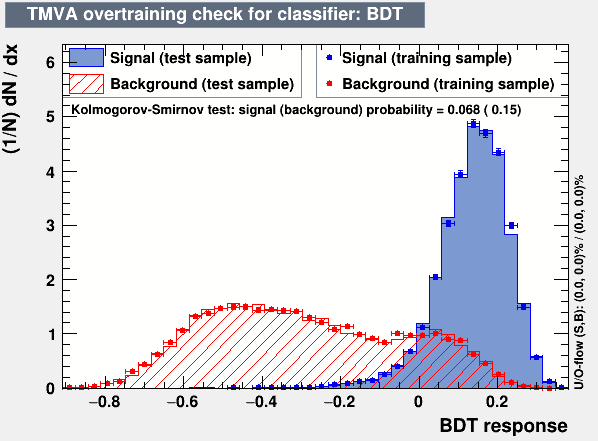
\includegraphics[width=7.5cm]{training&testing/overtraining_3_4.png}
        \captionof{figure}{Distribuzione dei dati del training (con i punti e relativi errori) e del testing (con i rettangoli) al variare della BDTresponse per il bin di $p_T$ [3,4]}
        \label{fig:testing_3_4}
        \end{flushleft}
        \end{minipage}
    ~
    \begin{minipage}{0.5\textwidth}
        \begin{flushright} \large
        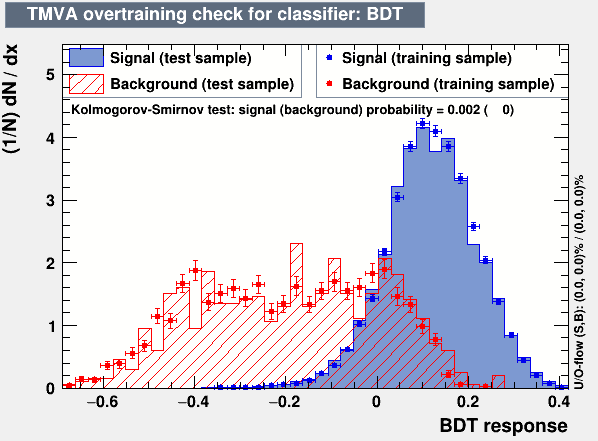
\includegraphics[width=7.5cm]{training&testing/overtraining_6_8.png}
        \captionof{figure}{Distribuzione dei dati del training (con i punti e relativi errori) e del testing (con i rettangoli) al variare della BDTresponse per il bin di $p_T$ [6,8]}
        \label{fig:testing_6_8}
        \end{flushright}
    \end{minipage} \\[1.cm]
    
Come si vede dai grafici \ref{fig:testing_3_4} e \ref{fig:testing_6_8} le distribuzioni dei dati per il training e per il testing coincidono quasi completamente considerando le barre di errore. 